\documentclass[a4paper,11pt]{article}
%\usepackage{epsf}
\usepackage{epsfig}
\usepackage{graphics}
\usepackage{amsmath}
%define the title
\title{Solutions to Practice Final \\ Math 21A}
\author{Ernest Woei}
\begin{document}
%generates the title
\maketitle

\paragraph{Problem 1} Use differentials to approximate $\log_2(\ln(e+1))$. \\
\textbf{Solution:} \\
Recall: $f(x+h) \approx f(x) + h*f ' (x)$ \emph{for small h}. \\
First we will approximate
\begin{center}
$\ln(e+1)$
\end{center}
Let $f(x)=\ln(x)$, then $f'(x)=\frac{1}{x}$. \\ \\
Choose: $x = e$ and $h = 1$ since differentials work \emph{for small h} and $1 < e$.  Therefore 
\begin{center}
$f(e+1) \approx f(e) + 1*f'(e) = \ln(e) + 1*\frac{1}{e} = 1 + \frac{1}{e}$
\end{center}
We will now approximate
\begin{center}$\log_2(1+\frac{1}{e})$\end{center}
Let $f(x) = \log_2(x)$, then $f'(x) = \frac{1}{\ln(2)*x}$. \\ \\
Choose $x = 1$ and $h = \frac{1}{e}$, then
\begin{center}$f(1+\frac{1}{e}) \approx f(1) + \frac{1}{e}*f ' (1) = \log_2(1) + \frac{1}{e}*\frac{1}{\ln(2)} \approx 0.5307$\end{center}
Therefore,
\begin{center}$\log_2(\ln(e+1)) \approx 0.5307$\end{center}
I computed (with a calculator) $\log_2(\ln(e+1)) \approx 0.3931$

\newpage
\paragraph{Problem 2} Find the slope of the tangent line at $(\frac{1}{2}, 2)$ to the curve:

\begin{center}$arctan(xy) = \frac{\pi}{4}\frac{1}{xy}$\end{center}
\textbf{Solution:} \\
Doing \emph{Implicit Differentiation}, we get 

\begin{center}
$\frac{d}{dx}\left(arctan(xy) = \frac{\pi}{4}\frac{1}{xy}\right) 
\Leftrightarrow 
\frac{1}{1+(xy)^2} \left(y + x\frac{dy}{dx}\right) = \frac{\pi}{4}\left(\frac{-y - x\frac{dy}{dx}}{(xy)^2}\right)$ \\
\end{center}
Substituting $x = \frac{1}{2}, y = 2$,
\begin{center}
$\frac{dy}{dx} = \frac{1+\frac{\pi}{2}}{-\frac{1}{4}-\frac{\pi}{8}}$
\end{center}

\paragraph{Problem 3}
Study the function $f(x) = x - \ln(x) + x^{-1}$
\paragraph{(a)} Compute the derivative and find extrema, if any. \\ \\
\textbf{Solution:} \\
$f ' (x) = 1 - \frac{1}{x} - x^{-2} = \frac{x^2 - x - 1}{x^2}$ \\
Set $f ' (x) = 0$, and solve for $x$. \\
Therefore $x = \frac{1 \pm \sqrt{5}}{2}$ (by quadratic formula on the
numerator of $f ' (x)$). \\
But $x$ must be positive, since $\ln(x)$ is defined for all $x > 0$. \\
Thus $x = \frac{1 + \sqrt{5}}{2}$.

\paragraph{(b)} Compute the second derivative and find inflection points.
\\ \\
\textbf{Solution:} \\
$f ''(x) = \frac{1}{x^2} + \frac{2}{x^3} = \frac{x+2}{x^3}$ \\ 
Set $f ''(x) = 0$ and solve for x. \\
Thus $x = -2$, but f(-2) is not defined, so there are no inflection points.

\newpage

\paragraph{Problem 4} Differentiate the functions (no need to simplify):
\paragraph{(a)}
$f(x) = \frac{x}{1+2^x}$ \\ \\
\textbf{Solution:}
\begin{center}$f ' (x) = \frac{1+2^x - x\ln(2)2^x}{(1+2^x)^2}$\end{center}

\paragraph{(b)} $sin(x)^{cos(x)}$ \\ \\
\textbf{Solution:} \\
Let $y = sin(x)^{cos(x)}$, then \\
$\ln(y) = ln(sin(x)^{cos(x)}) = cos(x)*\ln(sin(x))$ \\
Doing implicit differentiation: \\
$\frac{1}{y}\frac{dy}{dx} = \frac{cos^2(x)}{sin(x)} - sin(x)\ln(sin(x))$ \\
Thus $\frac{dy}{dx} = \left( \frac{cos^2(x)}{sin(x)} - sin(x)\ln(sin(x))\right) sin(x)^{cos(x)}$

\paragraph{(c)} $f(x) = tan(x)arcsin(x)$ \\ \\
\textbf{Solution:}
\begin{center}$f ' (x) = sec^2(x)*arcsin(x) +
\frac{tan(x)}{\sqrt{1-x^2}}$\end{center}

\paragraph{Problem 5} Evaluate the following limits using any method:
\paragraph{(a)}
\begin{displaymath}
\lim_{x \to \infty} \left( 1 +\frac{1}{2\sqrt{x}}\right)^{3\sqrt{x}}
\end{displaymath}

\paragraph{Solution:}
\begin{displaymath}
Recall: \lim_{x \to \infty} \left( 1 +\frac{1}{x}\right)^x = e
\end{displaymath}
Thus, \\
\begin{displaymath}
\lim_{x \to \infty} \left( 1 +\frac{1}{2\sqrt{x}}\right)^{3\sqrt{x}} = 
\lim_{x \to \infty} \left( 1 +\frac{1}{2\sqrt{x}}\right)^{3\sqrt{x} * \frac{2}{2}} = 
\lim_{x \to \infty} \left( 1 +\frac{1}{2\sqrt{x}}\right)^{2\sqrt{x} * \frac{3}{2}} = e^{\frac{3}{2}}
\end{displaymath}

\newpage
\paragraph{(b)}
\begin{displaymath}
\lim_{x \to 0^+} \frac{e^x-1}{\ln{x}}
\end{displaymath}

\textbf{Solution:}
\begin{displaymath}
\lim_{x \to 0^+} ln{x} = -\infty \\
\end{displaymath}

\begin{displaymath}
\lim_{x \to 0^+} e^x-1 = 0. \\
\end{displaymath}

\begin{displaymath}
Therefore \lim_{x \to 0^+} \frac{e^x-1}{\ln{x}} = 0.
\end{displaymath}

\paragraph{Problem 6} Consider the function $f(x) = 2^{3+\log_4{x^5}}-6$

\paragraph{(a)} Use $f'$ to show that $f$ is a one-to-one function on $[1,\infty)$ \\ \\
\textbf{Solution:} \\
$f'(x) = \ln(2)*2^{(3+\log_4{x^5})}(\frac{5x^4}{x^5*\ln{4}})$ \\
Since $x$ is in $[1, \infty)$ then $\log_4{x} \geq 0$.  Therefore $f ' (x) > 0$.
Thus f is one-to-one.

\paragraph{(b)} Find the inverse function $f^{-1}$ for $f$ (you do not need
to simplify). \\ \\
\textbf{Solution: } \\
Since $f$ is one-to-one then $f^{-1}$ exist, in this case we can swap $f(x)$
and $x$ for our initial problem and solve for $f(x)$ which will be our $f^{-1}$. \\
$f^{-1}(x) = (4^{\log_2{x+6}-3})^{\frac{1}{5}}$

\paragraph{Problem 7} Simplify as much as possible:
$2^{\log_4{\frac{1}{3}+\log_4{48}}}$ \\
\textbf{Solution: } \\
Using log rules: \\
$2^{\log_4{\frac{1}{3}+\log_4{48}}} = 2^{\log_4{\frac{48}{3}}} = 2^{\log_4{16}} = 2^2 = 4$

\newpage

\paragraph{Problem 8} Sketch a graph of a differentiable function f that
satisfies the following $f ' (x) = 0$ only when $x = 1$ or $4$; $f(1) = 3,
f(4) = 1$; $f ' (x) < 0$ for $x < 1$ and $f ' (x) > 0$ for $x > 4$ and $f '' (x) > 0$ when $x < 1$ \\ \\
\textbf{Solution: } \\ \\
This is a rough sketch, I couldn't draw it well.
\begin{figure}[h]
\begin{center}
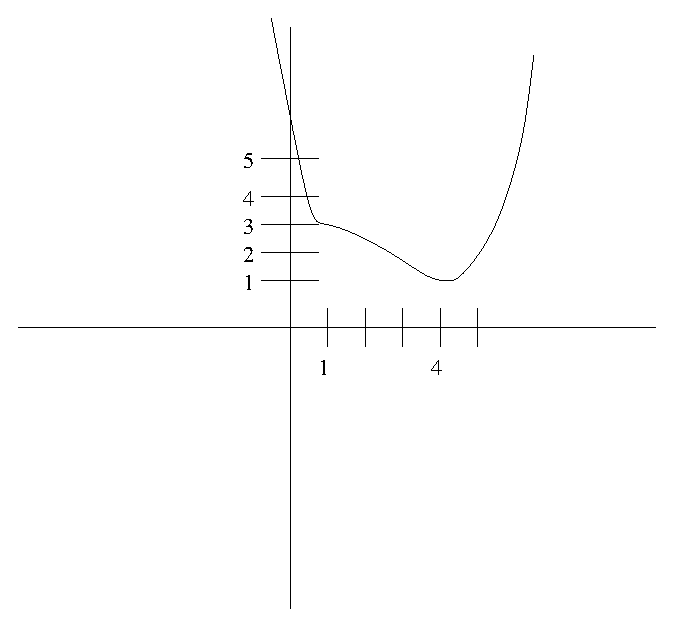
\epsfig{file=problem8.eps, height=2.25in}
\end{center}
\end{figure}

\paragraph{Problem 9} The stiffness of a rectangular beam is proportional to
the product of the width and the cube of the height of its cross section.
What shape beam should be cut from a log in the form of a right circular
cylinder of radius r in order to maximize its stiffness? \\ \\

\textbf{Solution: } \\ \\
We want to find the dimensions of the rectangular cross section of the beam that maximizes the stiffness.  That ractangle should be circumscribed in a circle of radius $r$, where $r$ is a constant throughout this problem.\\ \\
Let $h = $ height, and $w = $ width of the ractangular cross section.  By the Pythagorean Theorem, $$ \left( \frac{1}{2}h \right)^2 + \left( \frac{1}{2}w \right)^2 = r^2,$$ so $h^2 + w^2 = 4r^2$, and we get $w = \sqrt{4 r^2 - h^2}$. 
\\ \\
The stiffness is given by the function $y = w h^3$, so we have 
$$
y = (\sqrt{4 r^2 - h^2}) h^3.
$$
To maximize $y$, first find the derivative of $y$:
\begin{eqnarray*}
y' &=& \frac{-2h}{2\sqrt{4 r^2 - h^2}} ~ h^3 + \sqrt{4 r^2 - h^2} (3h^2) \\
&=& -h^4 +(4 r^2 - h^2)(3h^2) \\
&=& -h^4 + 12r^2 h^2 - 3h^4 \\
&=& 12r^2 h^2 - 4 h^4.
\end{eqnarray*}
Then solving $y'=0$ gives:
\begin{eqnarray*}
12r^2 h^2 - 4 h^4 &=& 0 \\
4 h^2 (3 r^2 - h^2) &=& 0 \\
h = 0 \mbox{~or~} h = \sqrt{3} r  
\end{eqnarray*}
Since $h=0$ gives zero stiffness, it cannot be the desired maximum stiffness.  Hence, the height must be $\sqrt{3} r$ and the width is $w = \sqrt{4 r^2 - h^2} = \sqrt{4 r^2 - 3 r^2} = r$.

\paragraph{Problem 10} A cannonball is fired from the ground straight up
into the air at a velocity of 336 feet per second.  Assuming constant
acceleration due to gravity is 16 feet per second, write an equation
describing the position of the cannonball after t seconds.  Find the time
that it hits the ground. \\ \\

\textbf{Solution: } \\ \\
$f(t) = -8t^2 + 336t$ \\
$f(t) = 0 \Rightarrow t = 42$ seconds

\paragraph{Problem 11} Using the limit definition of the derivative, show
that the function $f(x) = |x|$ is not differentiable at $x = 0$. \\ \\
\textbf{Solution: } \\ \\
Recall: \\
\begin{displaymath}
f'(x) = \lim_{\triangle x \to 0}\frac{f(x+\triangle x) - f(x)}{\triangle x}
\end{displaymath}
Note: \\
\begin{equation}
|x|=
  \begin{cases}
    x & \text{if $x\ge0$}, \\
    -x & \text{if $x < 0$}.
  \end{cases}
\end{equation}
Therefore we need to compute the left and right hand limits,
\begin{displaymath}
f'(0) = \lim_{\triangle x \to 0^+}\frac{\triangle x}{\triangle x} = 1
\end{displaymath}
\begin{displaymath}
f'(0) = \lim_{\triangle x \to 0^-}\frac{-\triangle x}{\triangle x} = -1
\end{displaymath}
Thus $f$ is not differentiable at 0, since the limits from both sides do not
equal.

\newpage
\paragraph{Problem 12} Extra Credit: Evaluate
\begin{displaymath}
\lim_{x \to 0} \frac{e^{\frac{-1}{x^2}}}{x}
\end{displaymath}
\textbf{Solution: }
\begin{eqnarray*}
\lim_{x\rightarrow 0} \frac{e^{-\frac{1}{x^2}}}{x} 
&=& \lim_{x\rightarrow 0}\frac{\frac{1}{x}}{e^{\frac{1}{x^2}}} \\
&=& \lim_{x\rightarrow 0} \frac{-\frac{1}{x^2}}{-\frac{2}{x^3} ~ e^{\frac{1}{x^2}}}\mbox{~~(using L'Hopital's rule)}\\ 
&=& \frac{x}{2 e^\frac{1}{x^2}} \\
&=& 0 \\
&& \mbox{because the numerator goes to $0$ and the denominator goes to $\infty$.}
\end{eqnarray*}
\end{document}
